
\section*{Тренировочное задание, вариант 3}

Осуществить планирование проекта со следующими временными характеристиками:

\begin{figure}[h!]
	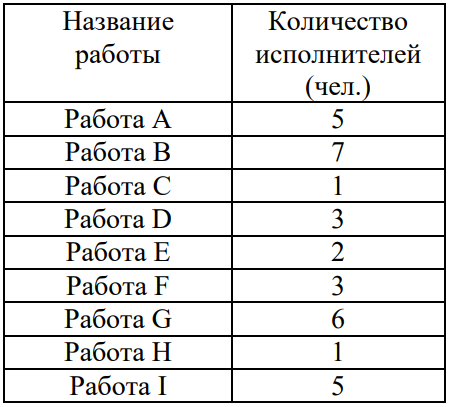
\includegraphics[scale=0.8, center]{train}
\end{figure}

Дата начала проекта – 1-й рабочий день марта текущего года.
Провести планирование работ проекта, учитывая следующие связи между задачами:

\begin{enumerate}
	\item Предусмотреть, что D – исходная работа проекта.
	\item Работа E следует за D.
	\item Работы A, G и C следуют за E.
	\item Работа B следует за A.
	\item Работа H следует за G.
	\item Работа F следует за C.
	\item Работа I начинается после завершения B, H, и F.
\end{enumerate}

Результат: 

\begin{figure}[h!]
	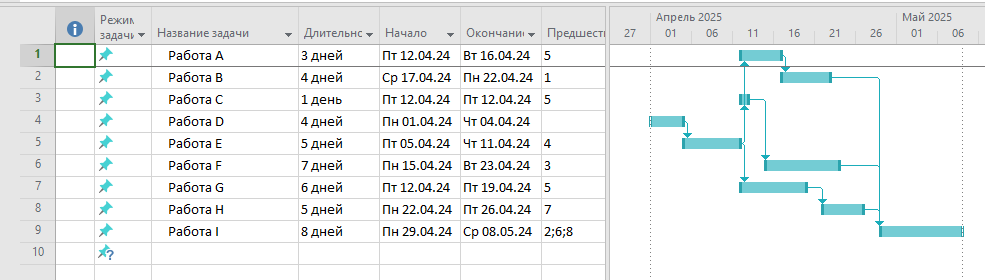
\includegraphics[scale=0.5, center]{train-result}
\end{figure}

\section*{Практическое задание}

Целью лабораторной работы №1 является освоение возможностей программы Microsoft Project для планирования проекта по разработке программного обеспечения.

\textbf{Содержание проекта:} команда разработчиков из 16 человек занимается созданием карты города на основе собственного модуля отображения. Проект должен быть завершен в течение 6 месяцев. Бюджет проекта: 50 000 рублей.


\subsection*{Задание 1}

На вкладке Проект (Сведения о проекте) выполним п.1 и п.6.

\begin{figure}[h!]
	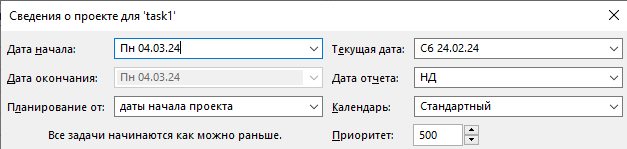
\includegraphics[scale=0.5, center]{task1_1}
\end{figure}

\clearpage

На вкладке Файл (Параметры, Расписание) выполним п. 2-5.

\begin{figure}[h!]
	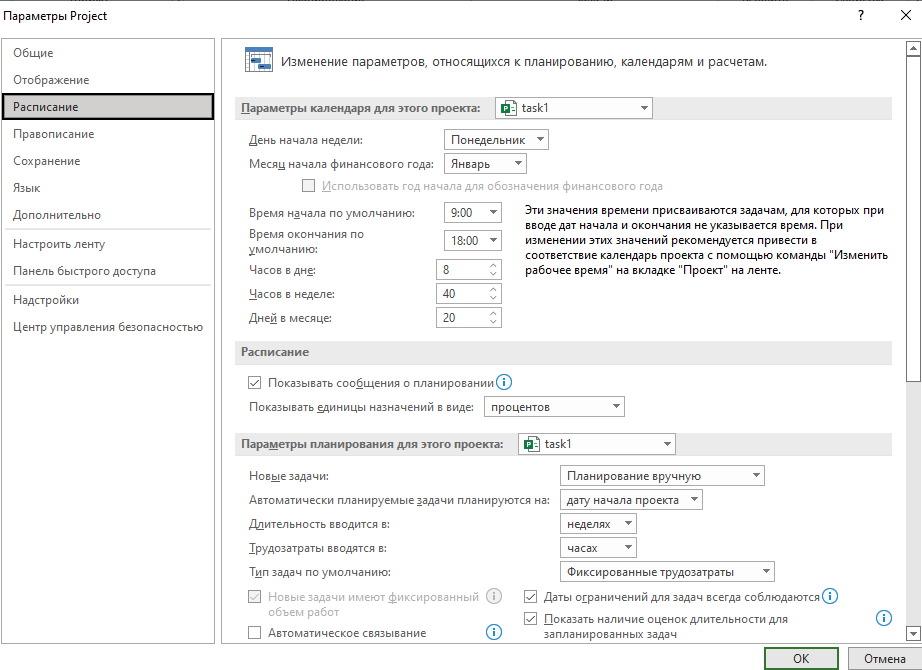
\includegraphics[scale=0.4, center]{task1_2}
\end{figure}

На вкладке Проект (Изменить рабочее время) добавим праздники на ближайшие 9 месяцев в календарь.

\begin{figure}[h!]
	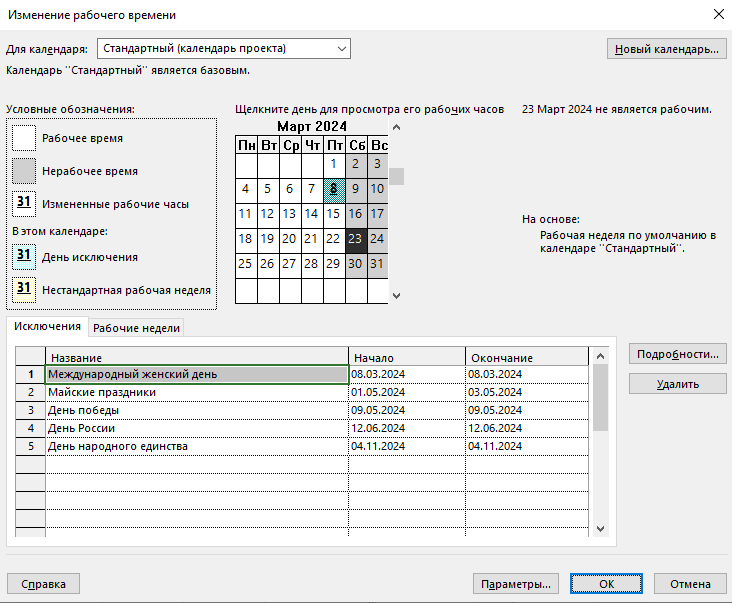
\includegraphics[scale=0.4, center]{task1_3}
\end{figure}

\clearpage

На вкладке Показать или скрыть добавим суммарную задачу проекта.

\begin{figure}[h!]
	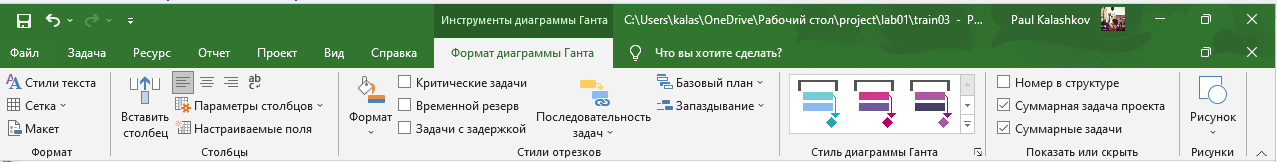
\includegraphics[scale=0.35, center]{task1_4}
\end{figure}

После этого отредактируем заметку о суммарной задаче:

\begin{figure}[h!]
	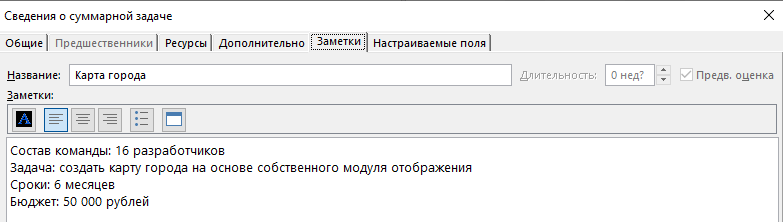
\includegraphics[scale=0.5, center]{task1_5}
\end{figure}

\subsection*{Задание 2}

Был осуществлён ввод задач.

\begin{figure}[h!]
	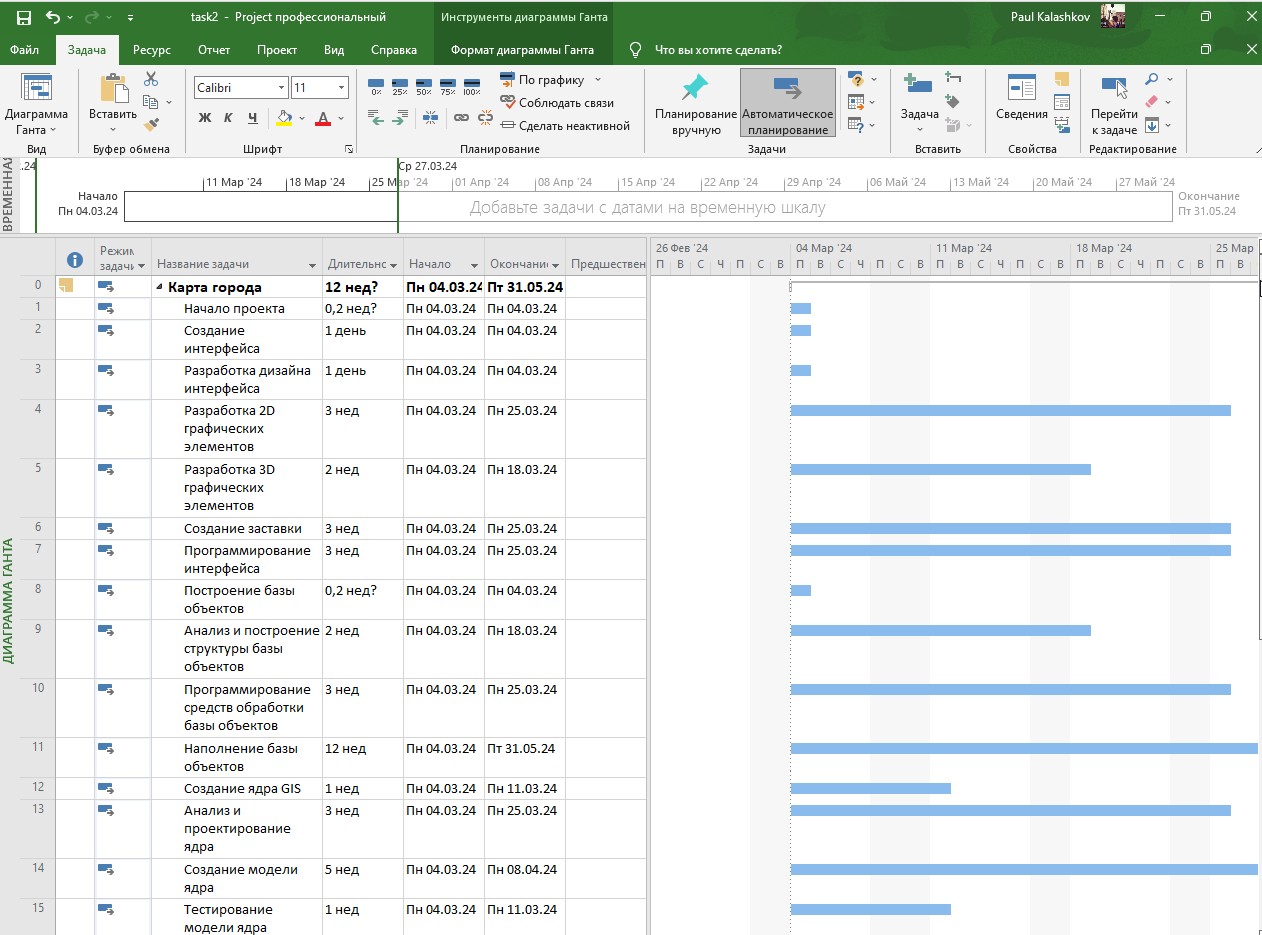
\includegraphics[scale=0.4, center]{task2}
\end{figure}
\clearpage

\subsection*{Задание 3}

При помощи кнопки на области Планирование задачи были разделены на подгруппы.

\begin{figure}[h!]
	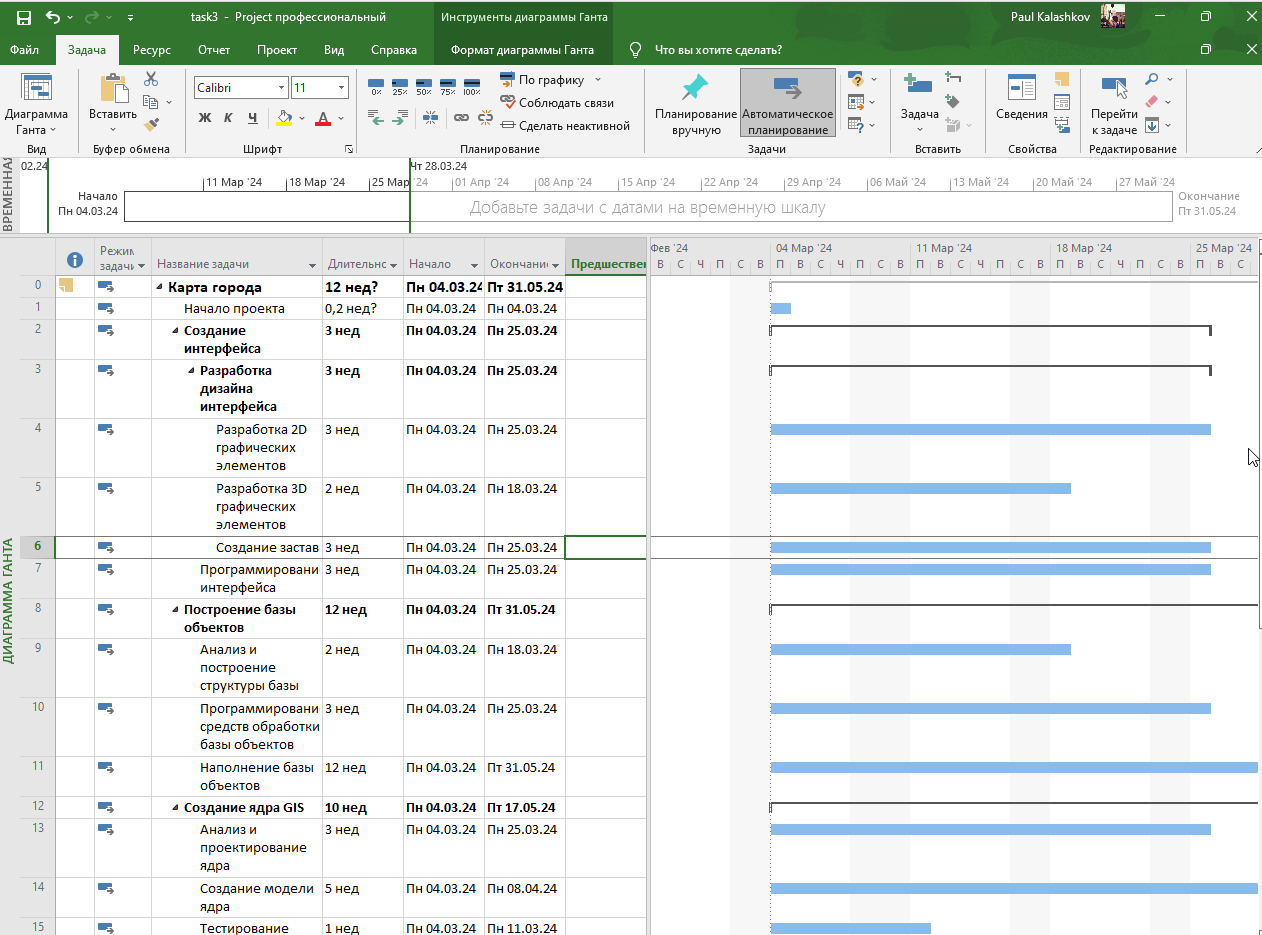
\includegraphics[scale=0.4, center]{task3}
\end{figure}
\clearpage

\subsection*{Задание 4}

Были добавлены связи между задачами посредством колонки Предшественники и получен итоговый результат:

\begin{figure}[h!]
	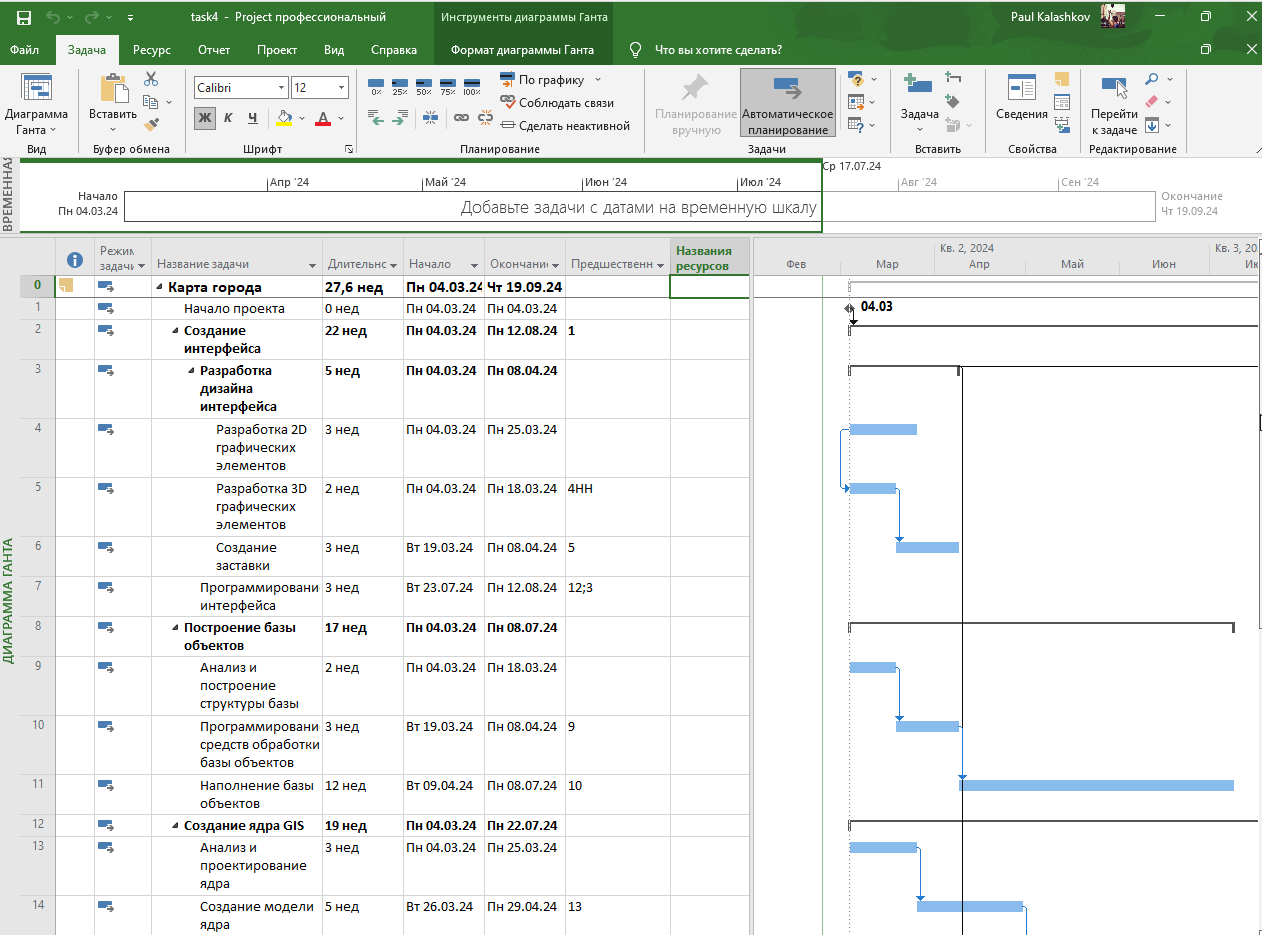
\includegraphics[scale=0.4, center]{task4_1}
\end{figure}

\begin{figure}[h!]
	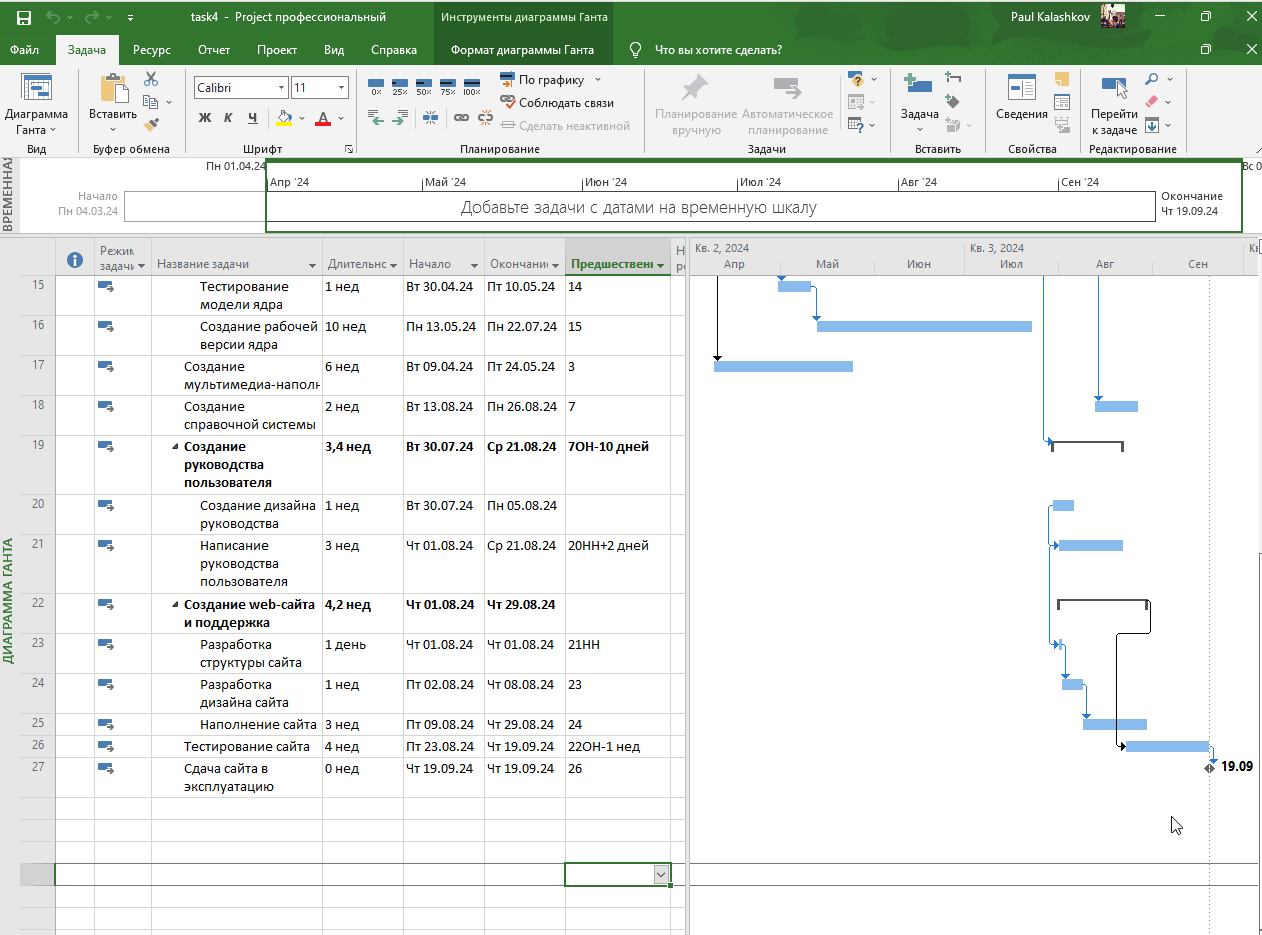
\includegraphics[scale=0.4, center]{task4_2}
\end{figure}

\clearpage

\section*{Заключение}

В ходе выполнения данной лабораторной работы была изучена программа MS Project 2016 и ряд её возможностей. Была проведена настройка рабочей среды, создание списка задач, их структурирование и установление связей между ними.

В результате выяснилось, что проект не укладывается в изначальные сроки: 19.09.2021 вместо 01.09.2021.
